\chapter{الفضاءات الجزئية، ومؤثرات الإسقاط، والقياس بوصفه تشابكًا}

لقد تركت مبرهنة بيل سؤالين مطروحين. ما الذي يبقى من التشابك عندما يُزعَج أحد عضوي الزوج، أو يُمتص، أو يُقاس؟ وما الذي يحوِّل، على وجه الدقة، تفاعلًا عاديًا إلى قياس؟ يمر الطريق إلى جواب عبر الجبر الخطي الأولي. فالخواص فضاءات جزئية، والاحتمالات قيم توقُّع لمؤثرات الإسقاط، وجهاز القياس نظام كمومي آخر تتشابك معه المنظومة.

\section{الدافع الافتتاحي: التشابك، والمحلية، والقياس}

فلنفترض أن حالة singlet قد فُصلت إلى جزأين متباعدين وقيس أحد الجزأين. فهل يجب على نظرية الحقل الكمومي أن تصف تبادلًا افتراضيًا بينهما؟ لا يحدث شيء يمكن كشفه على الجانب البعيد، ولا تصل إلى هناك أي رسالة قابلة للاستخدام. ويمكن تدوير أحد اللفين المغزليين محليًا بمجال مغناطيسي، بما يغيّر الصورة التفصيلية للحالة المشتركة، بينما يبقى مقدار التشابك ثابتًا تحت تلك العملية المحلية. وستأتي المقاييس الكمية للتشابك لاحقًا؛ أما النقطة المباشرة فهي أن نظامين لم يعودا يتفاعلان لا يمكنهما تغيير تشابكهما المشترك بمجرد عملية محصورة في أحد الجانبين.

\begin{classroomqa}
\lecturetimestamp{00:00:22}
\audiencequestion{هل يتطلب قياس أحد عضوي حالة singlet المفصولين فاصلًا من نوع المكان تبادلًا افتراضيًا ما مع الآخر؟}
\lecturerresponse{لا يحدث أي تبادل يمكن كشفه على الجانب الآخر. وقد تُدير عملية محلية أحد العاملين وتغيّر الصورة التي تُكتب بها الحالة المشتركة، لكنها لا تستطيع بذاتها أن ترسل رسالة أو أن تغيّر التشابك المتشارك عبر هذا الفصل.}
\end{classroomqa}

وهذا يفرض تصورًا أوسع لما يُعدُّ الشريك. فإذا سقط أحد عضوي زوج متشابك في ثقب أسود، فإن الآخر لا يكف عن كونه متشابكًا؛ بل يصبح متشابكًا مع درجات حرية الثقب الأسود، وبعد التبخر، مع الإشعاع المنبعث. والفكرة نفسها لا تحتاج إلى ثقب أسود. ألقِ أحد عضوي زوج متشابك في حوض استحمام ودعه يختلط بعنف بالماء. قد تضيع هويته الفردية في حالة الأجسام الكثيرة، ومع ذلك يبقى الجسيم البعيد متشابكًا مع حوض الاستحمام ككل، ثم في نهاية المطاف مع البخار المتصاعد.

هذه ليست قصة عن الاستمرار فحسب. إنها أيضًا قصة عن القابلية للعكس. فإذا كان التفاعل يستطيع أن يخلق تشابكًا، فإنه يستطيع، من حيث المبدأ، أن يفكَّه. فك التشابك ممكن، ولكن فقط عندما تعود الأنظمة إلى التماس وتتفاعل مرة أخرى. وكل ما يمكن أن يحدث في اتجاه يمكن أن يحدث في الاتجاه الآخر.

\begin{classroomqa}
\lecturetimestamp{00:04:45}
\audiencequestion{إذا قيس كلا اللفين المغزليين في زوج متشابك، فهل تبقى الإلكترونات متشابكة؟ وهل يمكن لقياس واحد وحده أن يفك تشابكها بالفعل؟}
\lecturerresponse{يمكن للقياسات أن تزيل التشابك المتبادل بينهما، وقد يكفي قياس واحد. ولكي نرى معنى هذا القول بدلًا من الاكتفاء بالقول بالانهيار، علينا أن نصف الرصد بوصفه تفاعلًا بين النظام وجهاز تسجيل.}
\end{classroomqa}

يحدد هذا السؤال الهدف: ربط الرصد، وانهيار الحزمة الموجية، والتشابك. لكن قبل الاقتراب منه، نحتاج إلى عرض أنظف للفضاءات الجزئية ولمؤثرات الإسقاط، من غير استعمال أدوات أثقل مما تتطلبه الحجة.

\section{البعد، والاعتماد الخطي، والأسس المتعامدة المعيارية}

ولذلك نبقى، في الوقت الراهن، مع فضاءات متجهية منتهية البعد مزودة بالبرا والكيت وبجداء داخلي. يبدأ سسكند بأبسط صورة ممكنة. فهو لا يعرّف البعد بعدّ المركبات في متجه عمودي. بل يعرّفه على نحو مجرد: بعد الفضاء المتجهي هو أكبر عدد من المتجهات المستقلة خطيًا يمكن العثور عليه فيه.

وبذلك تكون المجموعة \(\{|v_i\rangle\}\) مستقلة خطيًا عندما تفرض العلاقة
\begin{equation}
\sum_i c_i |v_i\rangle = 0
\end{equation}
أن تنعدم جميع المعاملات \(c_i\). وبصورة مكافئة، لا يمكن كتابة أي واحد من هذه المتجهات على أنه تركيب خطي من المتجهات الأخرى.

ومن الحاسم هنا أن التعامد ليس هو نفسه الاستقلال. ففي ثلاثة أبعاد قد تكون لدينا ثلاثة متجهات لا تعامد بينها إطلاقًا ومع ذلك تكون مستقلة خطيًا. وما يهم هو ما إذا كان يمكن بناء أحدها من الاثنين الآخرين. ومن جهة أخرى، في مستوًى ثنائي البعد لا بد أن يكون أي متجه ثالث في ذلك المستوى معتمدًا خطيًا على الأولين.

\begin{figure}[htbp]
\centering
\includegraphics[width=0.56\textwidth]{lecture_06_figure_02.png}
\caption{ثلاثة متجهات مرسومة على اللوح. تستخدم المحاضرة هذا الرسم للفصل بين فكرة التعامد وفكرة الاستقلال الخطي، ثم للتأكيد على أنه في مستوًى يكون المتجه الثالث معتمدًا على الأولين.}
\lectureframe{00:09:35}
\end{figure}

\begin{figure}[htbp]
\centering
\begin{tikzpicture}[scale=1.2]
\draw[->] (0,0) -- (2.3,0);
\draw[->] (0,0) -- (2.0,2.0);
\draw[->] (0.35,0.95) -- (1.05,1.45);
\fill (0,0) circle (1.2pt);
\end{tikzpicture}
\caption{إعادة بناء بالحد الأدنى لرسم اللوح. لا تحدد هذه اللقطة وحدها علاقةَ المعاملات الدقيقة؛ والنقطة الهندسية هي أنه في مستوًى ثنائي البعد لا يكون المتجه الثالث مستقلًا.}
\end{figure}

هذه هي مغزى الرسم. إذا كان الفضاء ثنائي البعد، فإن أكبر عدد من المتجهات المستقلة خطيًا هو اثنان. وإذا كان الفضاء ثلاثي البعد فهو ثلاثة. وعلى نحو أعم، إذا كان للفضاء بعد \(d\)، فعند إعطاء جداء داخلي يمكن إيجاد \(d\) متجهات وحدة متعامدة فيما بينها تمتده. وهذه هي متجهات الأساس. ويقول سسكند صراحة إنه لن يبرهن هذه المبرهنة هنا. وكل ما يريده هو النتيجة: متى وُجد مثل هذا الأساس أمكن توسيع كل متجه في الفضاء عليه.

\begin{classroomqa}
\lecturetimestamp{00:10:58}
\audiencequestion{هل يساوي عدد درجات الحرية المكانية بعد فضاء الحالات؟}
\lecturerresponse{لا. فالجسيم الذي يتحرك في غرفة له ثلاثة إحداثيات مكانية، لكنه يملك عددًا هائلًا من الحالات الكمومية المتعامدة فيما بينها. فبعد فضاء التهيئة وبعد فضاء هلبرت مفهومان مختلفان؛ ولا تُستخدم الأمثلة منتهية البعد هنا إلا لإظهار المنطق بوضوح.}
\end{classroomqa}

\section{التوسيع على الأساس، والديادات، وتحليل الهوية}

نختار الآن أساسًا متعامدًا معياريًا \(\{|n\rangle\}\)، بحيث يكون \(n=1,\dots,d\). وما على اللوح عند هذه النقطة واضح وموجز على نحو خاص:

\begin{figure}[htbp]
\centering
\includegraphics[width=0.62\textwidth]{lecture_06_figure_03.png}
\caption{أساس متعامد معياري وتوسيع حالة اعتباطية.}
\lectureframe{00:14:15}
\end{figure}

نكتب
\begin{align}
\langle m|n\rangle &= \delta_{mn}, \\
|\psi\rangle &= \sum_n a_n |n\rangle.
\end{align}
وهنا فإن \(\delta_{mn}\) هو دلتا كرونيكر: فهو يساوي \(1\) عندما يكون \(m=n\)، ويساوي \(0\) خلاف ذلك.

\paragraph{اشتقاق مفصل.} تُستعاد المعاملات بالإسقاط على الأساس. نضرب من اليسار بـ \(\langle m|\):
\begin{align}
\langle m|\psi\rangle
  &= \sum_n a_n \langle m|n\rangle \\
  &= \sum_n a_n \delta_{mn} \\
  &= a_m.
\end{align}
ومن ثم فإن المعاملات ببساطة هي
\begin{equation}
a_m = \langle m|\psi\rangle.
\end{equation}
والمعامل عدد عقدي عادي، لذلك يمكن وضعه على أي من جانبي الكيت من غير أن يتغير شيء.

إذا عوضنا المعامل مرة أخرى في التوسيع حصلنا على
\begin{equation}
|\psi\rangle = \sum_n |n\rangle \langle n|\psi\rangle.
\end{equation}
وهذا يوحي بأن الكائن \(|n\rangle\langle n|\)، وبوجه أعم \(|a\rangle\langle b|\)، ينبغي أن يُقرأ بوصفه مؤثرًا. وهذه هي الخطوة التالية بالضبط. ويؤثر الدياد وفقًا لـ
\begin{equation}
\bigl(|a\rangle\langle b|\bigr)|\psi\rangle = \langle b|\psi\rangle\,|a\rangle.
\end{equation}
فالبرا تستخرج عددًا عقديًا، والكيت تزود الاتجاه الناتج. وهذا هو الطريق البسيط عند سسكند للانتقال من المتجهات إلى المؤثرات.

والآن اقرأ التوسيع السابق قراءةً على مستوى المؤثرات. وبما أن
\begin{equation}
|\psi\rangle = \left(\sum_n |n\rangle\langle n|\right)|\psi\rangle
\end{equation}
لكل \(|\psi\rangle\)، فلا بد أن يكون المؤثر داخل القوسين هو مؤثر الهوية:
\begin{equation}
\sum_n |n\rangle\langle n| = I.
\end{equation}
وهذا هو تحليل الهوية.

\begin{figure}[htbp]
\centering
\includegraphics[width=0.60\textwidth]{lecture_06_figure_07.png}
\caption{الصيغة المكتملة لتحليل الهوية على اللوح.}
\lectureframe{00:18:30}
\end{figure}

\begin{classroomqa}
\lecturetimestamp{00:18:39}
\audiencequestion{هل يجب أن تشكّل المتجهات في تحليل الهوية أساسًا؟}
\lecturerresponse{نعم. فقد استعمل الاشتقاق كلاً من التطبيع والتعامد المتبادل، ويجب أن يجري الجمع على أساس كامل. ومجموعة اعتباطية من المتجهات لا تعطي تحليلًا للهوية.}
\end{classroomqa}

ومؤثر الهوية هو نفسه مؤثر الإسقاط على الفضاء كله. فكل متجه هو متجه ذاتي لـ \(I\)، وكل قيمة ذاتية هي \(+1\).

\begin{classroomqa}
\lecturetimestamp{00:19:14}
\audiencequestion{هل يفيد تحليل الهوية أن لكل متجه قيمة ذاتية تساوي واحدًا؟}
\lecturerresponse{نعم، بالنسبة إلى مؤثر الهوية. فهو استثنائي من حيث إن كل متجه هو متجهه الذاتي وأن \(I|\psi\rangle=|\psi\rangle\) لكل حالة.}
\end{classroomqa}

\section{الخواص بوصفها فضاءات جزئية ومؤثرات إسقاط}

وبهذه الأدوات في اليد، تُجري المحاضرة تصحيحها المفهومي المركزي. فالخاصية من قبيل \(k=\lambda\) ليست، على العموم، متجهًا واحدًا. بل هي فضاء جزئي كامل.

لتكن \(k\) كمية مرصودة هيرميتية، ولنفرض أن
\begin{equation}
k|A\rangle = \lambda |A\rangle, \qquad
k|B\rangle = \lambda |B\rangle,
\end{equation}
حيث إن \(|A\rangle\) و\(|B\rangle\) مستقلان خطيًا. عندئذ يكون لأي تركيب خطي القيمة الذاتية نفسها:
\begin{align}
k\bigl(\alpha|A\rangle+\beta|B\rangle\bigr)
  &= \alpha k|A\rangle + \beta k|B\rangle \\
  &= \alpha \lambda |A\rangle + \beta \lambda |B\rangle \\
  &= \lambda\bigl(\alpha|A\rangle+\beta|B\rangle\bigr).
\end{align}
ومن ثم فإن الفضاء الذاتي الموافق لـ \(\lambda\) مغلق تحت الجمع والضرب بعدد قياسي. إنه فضاء متجهي جزئي.

وأول مثال ملموس في المحاضرة هو نظام ذو لفين مغزليين. فالحالتان
\begin{equation}
|ud\rangle,\qquad |uu\rangle
\end{equation}
لهما قيمتان مختلفتان للَّف المغزلي الثاني، لكن القيمة نفسها للأول: فاللف المغزلي الأول إلى أعلى في كلتا الحالتين. لذلك فهما تولِّدان الفضاء الجزئي الذي فيه \(\sigma_3=+1\) للَّف المغزلي الأول.

\begin{figure}[htbp]
\centering
\includegraphics[width=0.46\textwidth]{lecture_06_figure_04.png}
\caption{حالتان في نظام ذي لفين مغزليين يكون فيهما اللف المغزلي الأول إلى أعلى.}
\lectureframe{00:23:27}
\end{figure}

هذه هي النقطة التي يجدر الاحتفاظ بها: فالخاصية ليست بالضرورة حالة واحدة. إنها مجموعة كاملة من الحالات ذات القيمة الذاتية نفسها.

لتجنب الالتباس في الترميز الذي يظهر لوهلة على السبورة، سنُبقي الأحرف الكبيرة \(A,B,\dots\) للمتجهات الذاتية المعينة، ونستعمل الأحرف الصغيرة \(a,b,\dots\) كمؤشرات جمع تجري على أساس متعامد مطبَّع للفضاء الجزئي الذاتي. فإذا كان \(\{|a\rangle\}\) مثل هذا الأساس للفضاء الجزئي \(k=\lambda\)، فإن مؤثر الإسقاط على ذلك الفضاء الجزئي هو
\begin{equation}
\Pi_{k=\lambda}=\sum_a |a\rangle\langle a|.
\end{equation}
وهذا ليس إلا مؤثر الهوية مقيَّدًا بذلك الفضاء الجزئي. فإذا كان \(|\psi\rangle\) يقع أصلًا في ذلك الفضاء الجزئي، فإن المسقِّط يعيده من دون تغيير. وإذا كان \(|\psi\rangle\) يقع جزئيًا خارجَه، فإن المسقِّط يطرح الباقي المتعامد ولا يُبقي إلا المركبة الموجودة في داخله.

\section{مسلّمة الاحتمال، والخصائص المتوافقة، ومراجعة Bell}

ما إن يُعاد تفسير الخصائص على أنها فضاءات جزئية حتى تتخذ مسلّمة الاحتمال أنقى صيغها. إذا كان \(|\psi\rangle\) مطبَّعًا، فإن احتمال امتلاكه الخاصية \(k=\lambda\) هو
\begin{equation}
P(k=\lambda)=\langle\psi|\Pi_{k=\lambda}|\psi\rangle.
\end{equation}

\begin{figure}[htbp]
\centering
\includegraphics[width=0.58\textwidth]{lecture_06_figure_05.png}
\caption{المسقِّط على الفضاء الجزئي الذاتي \(k=\lambda\). يهيئ ترتيب السبورة الخطوة التالية بالفعل: ضع المسقِّط بين \(\langle\psi|\) و\(|\psi\rangle\).}
\lectureframe{00:31:09}
\end{figure}

أدخل الصيغة الديادية للمسقِّط:
\begin{align}
P(k=\lambda)
  &= \left\langle \psi \left| \sum_a |a\rangle\langle a| \right| \psi \right\rangle \\
  &= \sum_a \langle\psi|a\rangle\langle a|\psi\rangle \\
  &= \sum_a |\langle a|\psi\rangle|^2.
\end{align}
وهذا هو بالضبط تفسير المحاضرة: فالاحتمال الكلي للخاصية هو مجموع احتمالات جميع الطرق المتعامدة التي يمكن أن تتحقق بها.

بالنسبة إلى كون اللف المغزلي الأول إلى الأعلى في منظومة ذات لفّين مغزليين، فإن الفضاء الجزئي المعني تولِّده \(|uu\rangle\) و\(|ud\rangle\)، ومن ثم
\begin{equation}
\Pi_{\sigma_3=+1}=|uu\rangle\langle uu|+|ud\rangle\langle ud|.
\end{equation}
وفي اختزال المحاضرة يُكتب هذا أيضًا على الصورة
\begin{equation}
\Pi_{\sigma_3=+1}=\frac{1+\sigma_3}{2},
\end{equation}
مع حذف مؤثر الهوية على اللف المغزلي الثاني.

\begin{classroomqa}
\lecturetimestamp{00:33:04}
\audiencequestion{ما الفرق بين المرصود والخاصية والمسقِّط؟}
\lecturerresponse{المرصود هو المؤثر الهرميتي \(k\). وتمثَّل الخاصية \(k=\lambda\) بفضائها الجزئي الذاتي، وتعني أن قياس \(k\) سيعطي على اليقين \(\lambda\). أما المسقِّط \(\Pi_{k=\lambda}\) فيعزل ذلك الفضاء الجزئي، وتعطي قيمة توقعه احتمال وجود الخاصية.}
\end{classroomqa}

\begin{classroomqa}
\lecturetimestamp{00:34:07}
\audiencequestion{هل يجب أن يكون المتجهان الذاتيان المنحلان \(A\) و\(B\) متعامدين أصلًا، وهل يشكّلان أساسًا للفضاء كله؟}
\lecturerresponse{لا يلزم أن تكون المتجهات الذاتية الأصلية متعامدة، لكن يمكن دائمًا اختيار أساس متعامد مطبَّع داخل فضائها الجزئي الذاتي. وهو أساس لذلك الفضاء الجزئي وحده؛ وتلزم اتجاهات متعامدة إضافية لبسط الفضاء الكامل. إن الإسقاط على كل متجه أساس في ذلك الفضاء الجزئي ثم جمعه يعطي الإسقاط على الفضاء الجزئي.}
\end{classroomqa}

\begin{classroomqa}
\lecturetimestamp{00:35:33}
\audiencequestion{هل يعني الرمز \(a\) في \(k|A\rangle=\lambda|A\rangle\) الشيء نفسه الذي يعنيه \(a\) الجاري الجمع عليه في المسقِّط؟}
\lecturerresponse{لا. فالأول يدل على متجه ذاتي معيّن، في حين أن المؤشر الواقع تحت إشارة الجمع يمر على كل متجه في أساس متعامد مطبَّع للفضاء الجزئي الذاتي. ويمنع الترميز المتميز أن تُفهم تسمية ثابتة على أنها مؤشر جمع صوري.}
\end{classroomqa}

\begin{classroomqa}
\lecturetimestamp{00:37:15}
\audiencequestion{هل الجداءات الداخلية في صيغة المسقِّط احتمالات أم سعات احتمال؟}
\lecturerresponse{كل \(\langle a|\psi\rangle\) هو سعة. والضرب في مرافقه المركب يعطي احتمالًا، وجمع تلك الاحتمالات على جميع الطرق المتعامدة لتحقيق \(k=\lambda\) يعطي الاحتمال الكلي للخاصية.}
\end{classroomqa}

ثم تسأل المحاضرة كيف نضم الخصائص بعضها إلى بعض. لنفترض أن لدينا خاصيتين متوافقتين، يمثلهما المسقِّطان المتبادلان \(P_k\) و\(P_\ell\). وبلغة المحاضرة، تُمثَّل عبارة AND بحاصل الضرب:
\begin{equation}
\Pi_{k=\lambda\,\wedge\,\ell=\mu}=P_kP_\ell=P_\ell P_k.
\end{equation}
والمنطق بسيط. فـ \(P_k|\psi\rangle\) يقع في الفضاء الجزئي \(k=\lambda\). وبما أن المؤثرين يتبادلان، فإن \(P_\ell P_k|\psi\rangle=P_kP_\ell|\psi\rangle\)، ولذلك يقع المتجه نفسه أيضًا في الفضاء الجزئي \(\ell=\mu\). وهكذا فإن حاصل الضرب يُسقِط على الخاصية المشتركة. أما الاحتمال المناظر فهو
\begin{equation}
P(k=\lambda,\ell=\mu)=\langle\psi|P_kP_\ell|\psi\rangle.
\end{equation}

تستحق الخطوة الأولى في تلك الحجة أن تُعرض مستقلة. فبالنسبة إلى أي حالة،
\begin{equation}
k\bigl(P_k|\psi\rangle\bigr)=\lambda P_k|\psi\rangle,
\end{equation}
ولذلك فإن \(P_k|\psi\rangle\) يقع في الفضاء الجزئي الذاتي \(k=\lambda\). وإذا كان \(P_k\) و\(P_\ell\) يتبادلان، أمكن كتابة حاصل الضرب مع أيٍّ من المسقِّطين على اليسار، ولذا فإنه ينتمي إلى كلا الفضاءين الجزئيين.

\begin{figure}[htbp]
\centering
\includegraphics[width=0.44\textwidth]{lecture_06_figure_06.png}
\caption{الحالة بعد الإسقاط بوصفها متجهًا في الفضاء الجزئي الذاتي.}
\lectureframe{00:41:57}
\end{figure}

\begin{figure}[htbp]
\centering
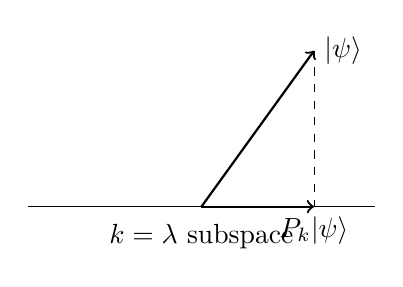
\begin{tikzpicture}[scale=1.1]
\draw (-2,0) -- (2,0);
\draw[->,thick] (0,0) -- (1.3,1.8) node[right] {$|\psi\rangle$};
\draw[dashed] (1.3,1.8) -- (1.3,0);
\draw[->,thick] (0,0) -- (1.3,0) node[below] {$P_k|\psi\rangle$};
\node at (0,-0.35) {$k=\lambda$ subspace};
\end{tikzpicture}
\caption{إسقاط متجه اعتباطي إلى الفضاء الجزئي الذاتي \(k=\lambda\).}
\end{figure}

\begin{figure}[htbp]
\centering
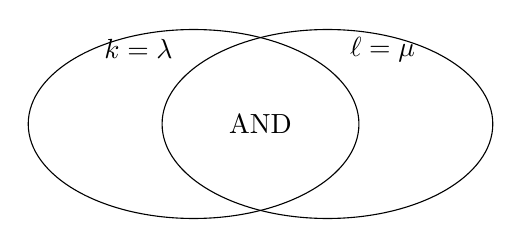
\begin{tikzpicture}[scale=1.0]
\draw (0,0) ellipse (2.1 and 1.2);
\draw (1.7,0) ellipse (2.1 and 1.2);
\node at (-0.7,0.95) {$k=\lambda$};
\node at (2.4,0.95) {$\ell=\mu$};
\node at (0.85,0) {AND};
\end{tikzpicture}
\caption{إعادة بناء لصورة الفضاءات الجزئية المتقاطعة الكامنة وراء عبارة AND للمسقِّطات المتبادلة.}
\end{figure}

\begin{figure}[htbp]
\centering
\includegraphics[width=0.66\textwidth]{lecture_06_figure_08.png}
\caption{الحجة المعروضة على السبورة التي تُظهر أن المسقِّطات المتبادلة تنتقي الفضاء الجزئي الذاتي المشترك.}
\lectureframe{00:45:20}
\end{figure}

\begin{classroomqa}
\lecturetimestamp{00:44:42}
\audiencequestion{هل الخاصية المشتركة هي نفسها التقاطع في المنطق الكلاسيكي؟}
\lecturerresponse{نعم. بالنسبة إلى المسقِّطات المتبادلة، فإن \(P_kP_\ell\) يُسقِط على تقاطع الفضاءين الجزئيين الذاتيَّين. وإذا كان هذا التقاطع لا يحتوي إلا على المتجه الصفري، فلا توجد حالة غير صفرية تمتلك الخاصيتين معًا.}
\end{classroomqa}

ومن باب الاستكمال، فإن المسقِّط على الفضاء الجزئي الموافق لعبارة OR للخاصيتين المتوافقتين هو
\begin{equation}
P_{k\lor\ell}=P_k+P_\ell-P_kP_\ell .
\end{equation}
وعندما تكون البدائل متنافية فيما بينها، يكون \(P_kP_\ell=0\)، ويختزل هذا إلى المجموع \(P_k+P_\ell\). وهذا الطرح أساسي كلما تراكب الفضاءان الجزئيان، لأن تقاطعهما يجب ألا يُحسب مرتين.

ويُربط مفهوم التوافق نفسه بعد ذلك بأمثلة فيزيائية. ففي منظومة ذات لفّين مغزليين، تتبادل أي مركبة \(\sigma_i\) من اللف المغزلي الأول مع أي مركبة \(\tau_j\) من الثاني:
\begin{equation}
[\sigma_i,\tau_j]=0.
\end{equation}
وعلى النقيض من ذلك، فإن المركبات المختلفة للَّف المغزلي نفسه لا تتبادل:
\begin{equation}
[\sigma_1,\sigma_3]\neq 0.
\end{equation}
ولهذا السبب يمكن قياس مركبة واحدة من كل من لفّين مغزليين منفصلين، لكن لا يمكن قياس مركبتين مختلفتين للَّف المغزلي نفسه في آن واحد.

\begin{classroomqa}
\lecturetimestamp{00:46:12}
\audiencequestion{ما الأمثلة الملموسة على المرصودات المتوافقة؟}
\lecturerresponse{أي مؤثر يؤثر في اللف المغزلي الأول يتبادل مع كل مؤثر يؤثر في الثاني، لأنهما يؤثران في عاملين تنسوريين مختلفين. ومركبات الموضع \(x,y,z\) أسرة متوافقة أخرى. وعلى النقيض من ذلك، فإن مركبتين مختلفتين للَّف المغزلي نفسه، أو الموضع وزخمه المقترن به، لا يتبادلان.}
\end{classroomqa}

\begin{classroomqa}
\lecturetimestamp{00:47:26}
\audiencequestion{هل يجب أن يعني النظام الفرعي جسيمًا مختلفًا؟}
\lecturerresponse{لا. إنه يعني مجموعة من درجات الحرية محددة بصورة مستقلة. وتعطي الجسيمات المتميزة أبسط العوامل التنسورية، لكن يمكن أيضًا معالجة درجات الحرية المختلفة لجسيم واحد على نحو منفصل عندما تسمح بذلك بنيتها المؤثرية.}
\end{classroomqa}

\begin{classroomqa}
\lecturetimestamp{00:48:37}
\audiencequestion{إذا كان هذا العدد الكبير من المؤثرات على أنظمة فرعية مختلفة يتبادل، فما مثال زوج بسيط غير متوافق؟}
\lecturerresponse{توفر مركبتان للَّف المغزلي نفسه المثال القياسي: \(\sigma_1\) و\(\sigma_3\) لا يتبادلان، لذلك لا يستطيع أي جهاز إسناد قيمتين محددتين بدقة لهما معًا. ومبدّل المصفوفات غير الصفري هو الاختبار الجبري.}
\end{classroomqa}

يعيد Susskind الآن تناول مبرهنة Bell. وهو لا يعيد حسابات المحاضرة السابقة، بل يعيد بناء منطقها باللغة الجديدة. والمتباينة الكلاسيكية، بصيغتها الاحتمالية، هي
\begin{equation}
P(A\wedge \neg B)+P(B\wedge \neg C)\ge P(A\wedge \neg C).
\end{equation}
وهذه مبرهنة في منطق المجموعات الكلاسيكي، لا في ميكانيكا الكم. وفي الحالة المفردة، يكون اللفان المغزليان متضادَّي الاتجاه على أي محور مشترك، ولذلك يمكن استبدال عبارة نفي تخص اللف المغزلي الأول بالعبارة الإيجابية المناظرة للثاني. وهذا يتيح إعادة كتابة المتباينة على أنها عبارة عن خصائص مشتركة في منظومة ذات لفّين مغزليين.

ومع حذف مؤثرات الهوية على العوامل غير المتأثرة، فإن مسقِّطات الخاصية المفردة التي تظهر في المحاضرة هي
\begin{equation}
\frac{1+\sigma_3}{2},\qquad
\frac{1+\frac{\tau_1+\tau_3}{\sqrt2}}{2},\qquad
\frac{1+\frac{\sigma_1+\sigma_3}{\sqrt2}}{2},\qquad
\frac{1+\tau_1}{2}.
\end{equation}
ولذلك فإن مسقِّطات الخصائص المشتركة الثلاثة ذات الصلة هي
\begin{align}
\Pi_1 &= \frac{1+\sigma_3}{2}\,\frac{1+\frac{\tau_1+\tau_3}{\sqrt2}}{2}, \\
\Pi_2 &= \frac{1+\frac{\sigma_1+\sigma_3}{\sqrt2}}{2}\,\frac{1+\tau_1}{2}, \\
\Pi_3 &= \frac{1+\sigma_3}{2}\,\frac{1+\tau_1}{2}.
\end{align}

\begin{figure}[htbp]
\centering
\includegraphics[width=0.68\textwidth]{lecture_06_figure_09.png}
\caption{اختيارات المحللات الثلاثة مكتوبةً على هيئة حاصل ضرب لمسقِّطات لفٍّ مغزلي واحد.}
\lectureframe{01:01:45}
\end{figure}

تتحدث المحاضرة عن الحالة المفردة بالصيغة السبورية المألوفة غير المطبَّعة
\begin{equation}
|\Psi_{\mathrm{singlet}}\rangle \propto |ud\rangle-|du\rangle.
\end{equation}
وتكفي هنا إشارة التناسب. فما يهم في المنطق هو الحالة نفسها، وبخاصة الإشارة النسبية، لا التطبيع الكلي. إن تقييم \(\langle \Pi_1\rangle+\langle \Pi_2\rangle\) في مقابل \(\langle \Pi_3\rangle\) في الحالة المفردة يعطي الانتهاك الذي جرى الحصول عليه في المحاضرة السابقة. والخلاصة المهمة هي التي يشدد عليها Susskind شفهيًا: ميكانيكا الكم ليست نظرية مجموعات كلاسيكية متنكرة.

\begin{classroomqa}
\lecturetimestamp{00:52:31}
\audiencequestion{إذا كان اللف المغزلي إلى الأعلى وإلى الأسفل متعامدين، فهل تعني الإشارة السالبة أن أحد الكيتين هو سالب الآخر؟}
\lecturerresponse{لا. \(|u\rangle\) و\(|d\rangle\) متجهان متعامدان ومتمايزان. وتنتمي الإشارة النسبية إلى تراكب مثل \(|ud\rangle-|du\rangle\) ويمكن أن تغيّر خواصه الفيزيائية؛ أما الإشارة الكلية التي تضرب الحالة كلها فلا أهمية لها.}
\end{classroomqa}

\begin{classroomqa}
\lecturetimestamp{00:53:06}
\audiencequestion{هل تُنتهك متباينة بيل لكل حالة كمومية ولكل اختيار للخواص؟}
\lecturerresponse{لا. كثير من الحالات وكثير من اختيارات المحاور تستوفي متباينة بيل معيّنة. ويتوقف الانتهاك على كل من الحالة والمرصودات المختارة. وتغيير الزوايا الوسطى والنهائية يغيّر ما إذا كان هذا الاختبار يكشف الارتباطات غير الكلاسيكية.}
\end{classroomqa}

\begin{classroomqa}
\lecturetimestamp{01:02:47}
\audiencequestion{ماذا يمكن أن نستنتج عندما تنتهك حالة معيّنة متباينة بيل هذه، أو يتصادف أن تستوفيها؟}
\lecturerresponse{يثبت الانتهاك أن الإحصاءات المرصودة لا يمكن أن تنشأ من منطق المجموعات الكلاسيكي المستخدم في الاشتقاق. أما استيفاء متباينة مختارة واحدة فلا يجعل الحالة كلاسيكية بحد ذاته، لأن اختيارًا آخر للخواص قد يكشف عن انتهاك.}
\end{classroomqa}

\section{المحلية بعد بيل}

حساب المؤثرات الإسقاطية ليس مجرد لعبة رمزية. تخيّل أننا نعدّ مرارًا أزواجًا مترابطة في الحالة الأرضية المفردة، ثم نفصل العضوين ونقسم الجماعة المحضَّرة على نحو متماثل إلى ثلاث مجموعات كبيرة. تقيس المجموعة الأولى الإعدادين \(0^\circ\) و\(45^\circ\)، والثانية الإعدادين \(45^\circ\) و\(90^\circ\)، والثالثة الإعدادين \(0^\circ\) و\(90^\circ\). وتقدّر التواترات في المجموعات الثلاث الاحتمالات الثلاثة في المتباينة.

\begin{classroomqa}
\lecturetimestamp{01:04:30}
\audiencequestion{ما الترتيب المختبري الذي تصفه فعليًا احتمالات بيل الثلاثة؟}
\lecturerresponse{ينتج مصدر كثيرًا من الأزواج المتشابكة المحضَّرة على نحو متماثل، ويرسل العضوين إلى محللين منفصلين. اقسم الأزواج إلى ثلاث جماعات، واستعمل في كل جماعة الزوج الموافق من اتجاهات المحللين. ويقدّر عدُّ النواتج المشتركة كلَّ احتمال. ويمكن فصل جسيم مشحون وجسيم مضاد له بواسطة مجال؛ غير أن اختبارات بيل العملية تستخدم الفوتونات بدلًا من ذلك في كثير من الأحيان.}
\end{classroomqa}

\begin{classroomqa}
\lecturetimestamp{01:08:00}
\audiencequestion{استخدم برهان المجموعات الكلاسيكي جماعة واحدة. فكيف يمكن لثلاث جماعات مقيسة على حدة أن تختبره؟}
\lecturerresponse{المتباينة عبارة عن بيان يتعلق بالاحتمالات كما يتعلق بالأعداد. فإذا كانت العينات الثلاث كلها مأخوذة من إجراء التحضير نفسه، فإن تواتراتها النسبية تقدّر التوزيعات الاحتمالية الثلاثة لجماعة مشتركة واحدة. والتحضير المتماثل هو الافتراض الذي لا غنى عنه.}
\end{classroomqa}

تؤدي هذه المراجعة لبيل مباشرة إلى القلق الفيزيائي الذي لا يزال مخيمًا على القاعة. إذا كانت الارتباطات حقيقية، فلماذا لا يمكن استخدامها لإرسال إشارة؟

\begin{classroomqa}
\lecturetimestamp{01:09:41}
\audiencequestion{لماذا لا يمكن استخدام الارتباطات المتشابكة لإرسال رسالة أسرع من الضوء؟}
\lecturerresponse{كل طرف على حدة لا يزال يرى متتالية عشوائية غير قابلة للتحكم. ولا يظهر الارتباط إلا عندما تُقارَن السجلّات عبر قناة كلاسيكية عادية. ومع ذلك، يرتب اختبار بيل الحاسم اختيارات القياس وعمليات الكشف بحيث لا يمكن لأي إشارة ضوئية أن تنتقل بين الطرفين في الوقت المناسب، وبذلك يستبعد آلية اتصال محلية لإنتاج الإحصاءات المشتركة.}
\end{classroomqa}

إذا انقضى وقت يكفي لانتقال إشارة ضوئية بين الجهازين، فإن الارتباط لا يناقض النسبية في حد ذاته؛ فقد يكون المرء قد اكتشف مجرد تأثير عادي لم يُنتبه إليه. والتجربة الحاسمة تسد هذا المنفذ. وبلغة بيل، يجب أن يكون أي وصف بالمتغيرات الخفية يعيد إنتاج الارتباطات غير محلي، لكن الاعتماد اللامحلي ليس هو الشيء نفسه الذي تمثله رسالة قابلة للتحكم تفوق سرعتها سرعة الضوء.

\begin{classroomqa}
\lecturetimestamp{01:12:18}
\audiencequestion{هل حفظ الزخم الزاوي أساسي في هذه الحجة؟}
\lecturerresponse{لا. فاللف المغزلي نموذج مناسب ذو حالتين، لا مكوّنًا مقدسًا. ويمكن لأي زوج من الأنظمة ثنائية المستوى يملك الحالة المتشابكة المطلوبة وأسُس قياس بديلة أن يُظهر البنية المنطقية نفسها.}
\end{classroomqa}

هذا النقاش لا يختتم المحاضرة؛ بل يمهّد الأرضية للتحول التالي. لقد علّمنا بيل أن ميكانيكا الكم ليست منطقًا كلاسيكيًا، لكن السؤال التالي مختلف. ما القياس، إجرائيًا ورياضيًا، وكيف يدخل في قصة التداخل؟

\section{تجربة الشقين ذات الحالات المنتهية، والتداخل، والقياس بوصفه تشابكًا}

تغيّر المحاضرة الآن النموذج. ينتقل Susskind إلى تجربة الشقين، لكنه يبسطها فورًا إلى مسألة ذات عدد منتهٍ من الحالات حتى يمكن استعمال أدوات فضاء المتجهات نفسها من دون استحضار الجهاز الكامل لميكانيكا الموجة على المتصل. وهو يقول حتى، في ما معناه، إن هذه ما تزال تجربة الشقين، ولكن بعد اختزالها إلى مجموعة صغيرة من حالات الأساس.

هناك حالة مصدر \(|0\rangle\)، وحالتا شقين \(|1\rangle\) و\(|-1\rangle\)، ومجموعة من حالات الشاشة \(|n\rangle\). وهذه \(|n\rangle\) متعامدة ومطبَّعة، لأن المواضع المختلفة على الشاشة هي تهيئات مختلفة. وتختار المحاضرة صراحةً ألا تتعقب التطبيع بدقة هنا. وتؤجَّل الوحدوية. وما يهم في هذه المرحلة هو الخطية.

\begin{figure}[htbp]
\centering
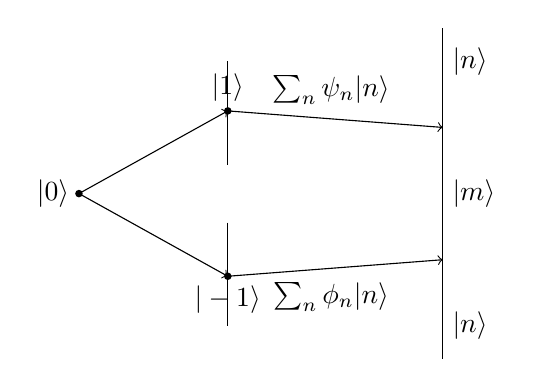
\begin{tikzpicture}[scale=1.05]
\fill (0,0) circle (1.3pt);
\node[left] at (0,0) {$|0\rangle$};

\draw (1.8,1.6) -- (1.8,0.35);
\draw (1.8,-0.35) -- (1.8,-1.6);
\fill (1.8,1) circle (1.3pt);
\fill (1.8,-1) circle (1.3pt);
\node[above] at (1.8,1) {$|1\rangle$};
\node[below] at (1.8,-1) {$|-1\rangle$};

\draw (4.4,2.0) -- (4.4,-2.0);
\node[right] at (4.4,1.6) {$|n\rangle$};
\node[right] at (4.4,0.0) {$|m\rangle$};
\node[right] at (4.4,-1.6) {$|n\rangle$};

\draw[->] (0,0) -- (1.8,1);
\draw[->] (0,0) -- (1.8,-1);
\draw[->] (1.8,1) -- (4.4,0.8);
\draw[->] (1.8,-1) -- (4.4,-0.8);

\node at (3.05,1.25) {$\sum_n \psi_n |n\rangle$};
\node at (3.05,-1.25) {$\sum_n \phi_n |n\rangle$};
\end{tikzpicture}
\caption{نسخة ذات حالات منتهية من تجربة الشقين: حالة المصدر \(|0\rangle\)، وحالتا الشقين \(|1\rangle\) و\(|-1\rangle\)، وأساس الشاشة \(|n\rangle\).}
\end{figure}

\begin{figure}[htbp]
\centering
\includegraphics[width=0.68\textwidth]{lecture_06_figure_10.png}
\caption{شبكة المواضع المنتهية إلى جانب قاعدة التطور الخطي \(A\to A'\)، \(B\to B'\).}
\lectureframe{01:18:00}
\end{figure}

بحكم التناظر، تتطور حالة المصدر إلى تراكب ذي سعتين متساويتين لحالتي الشقين:
\begin{equation}
|0\rangle \longrightarrow |1\rangle+|-1\rangle.
\end{equation}
ولنجعل الآن حالة الشق العلوي تتطور إلى
\begin{equation}
|1\rangle \longrightarrow \sum_n \psi_n |n\rangle,
\end{equation}
وحالة الشق السفلي إلى
\begin{equation}
|-1\rangle \longrightarrow \sum_n \phi_n |n\rangle.
\end{equation}
الأسهم هنا تعني تطورًا زمنيًا، لا مساواةً بين حالات في اللحظة نفسها. وبحسب الخطية،
\begin{equation}
|1\rangle+|-1\rangle \longrightarrow \sum_n (\psi_n+\phi_n)|n\rangle.
\end{equation}
تلك هي القاعدة الأساسية. تُجمع السعات قبل تكوين الاحتمالات.

\begin{classroomqa}
\lecturetimestamp{01:21:59}
\audiencequestion{كيف يمكن لحالة الشق \(|1\rangle\) أن تتحول إلى حالات موسومة أيضًا بأعداد صحيحة \(n\)؟ أهذه الكيتات في المكان والزمان نفسيهما؟}
\lecturerresponse{تشير العلامات إلى شرائح زمنية مختلفة. فـ \(|1\rangle\) يدل على الإلكترون عند الشق العلوي، في حين أن \(|n\rangle\) على اليمين تدل على مواضع لاحقة ممكنة على الشاشة. والسهم هو تطور زمني، لا مساواة بين تهيئات متزامنة.}
\end{classroomqa}

\begin{classroomqa}
\lecturetimestamp{01:25:30}
\audiencequestion{هل ينبغي تطبيع السعات، وهل تحمل وحدات فيزيائية؟}
\lecturerresponse{يجب على تطور كامل أن يحفظ الاحتمال الكلي؛ تلك هي الوحدوية. وهنا يُحذَف التطبيع المشترك لأن المهم فقط هو جمع سعات المسارات وإلغاؤها. ويمكن إعادة أي عوامل مقياس عندما تُطبَّع الحالة.}
\end{classroomqa}

ولذلك فإن احتمال الوصول إلى موضع الشاشة \(m\) هو
\begin{align}
P_m &= |\psi_m+\phi_m|^2 \\
    &= |\psi_m|^2 + |\phi_m|^2 + \psi_m^*\phi_m + \phi_m^*\psi_m.
\end{align}
الحدان الأولان هما ما كان سيُنتجه الاستدلال الكلاسيكي. أما الحدّان الأخيران فهما حدّا التداخل.

\begin{figure}[htbp]
\centering
\includegraphics[width=0.68\textwidth]{lecture_06_figure_11.png}
\caption{سعة الشاشة وتوسيع احتمالها إلى أربعة حدود على اللوح.}
\lectureframe{01:29:20}
\end{figure}

عند النقطة المتناظرة على الشاشة، ولنسمها \(m=0\)، يوحي التناظر بأن \(\psi_0=\phi_0\). وعندئذٍ
\begin{equation}
P_0 = |\psi_0+\phi_0|^2 = |2\psi_0|^2 = 4|\psi_0|^2.
\end{equation}
ينتج عن فتح الشقين معًا عند تلك النقطة احتمال يساوي أربعة أمثال احتمال الشق الواحد، لا مثليه. هذا هو التداخل البنّاء.

أدخل الآن إزاحة طور بحيث يكون \(\phi_0=-\psi_0\). وعندئذٍ
\begin{equation}
P_0 = |\psi_0-\psi_0|^2 = 0.
\end{equation}
كل شق على حدة يسمح بالوصول إلى تلك النقطة، لكن فتحهما معًا قد يجعل الوصول إليها مستحيلًا. هذا هو التداخل الهدّام. ويتوقف Susskind صراحةً عند مدى غرابة هذا الأمر: فهو، في تقديره، بالغ الغرابة بقدر غرابة بيل.

\begin{classroomqa}
\lecturetimestamp{01:33:14}
\audiencequestion{ماذا لو لم يُغيَّر مزيح الطور أو اختيار الشق إلا بعد أن يكون الإلكترون قد انطلق بالفعل؟ هل يحتاج الشق الآخر إلى وقت ليعلم بذلك؟}
\lecturerresponse{يعتمد الجواب على الترتيب الزمكاني الدقيق وعلى ما إذا كان الإلكترون يلاقي الجزء المعدَّل من الجهاز. تُطوِّر ميكانيكا الكم الحالة وفق الإعداد الفعلي؛ وتبقى الاحتمالات ناتجة من جمع السعات المنطبقة. ويجب تحديد مقترح الاختيار المتأخر بدقة قبل إمكان تقييم دعاوى المحلية.}
\end{classroomqa}

الآن ندخل الجهاز إلى الصورة. يوجد نظام إضافي واحد ذو حالتين، هو لفّ مغزلي يكون في البداية في الحالة \(|d\rangle\). إذا مر الإلكترون عبر الشق العلوي، فإنه يقلب ذلك اللف المغزلي إلى \(|u\rangle\). وإذا مر عبر الشق السفلي، فإنه يتركه بلا تغيير. والحالة المركبة الابتدائية هي \(|0,d\rangle\)، وتصبح قاعدة التحديث الأولى
\begin{equation}
|0,d\rangle \longrightarrow |1,u\rangle + |-1,d\rangle.
\end{equation}
ذلك السطر الواحد هو المعنى الكامل للقياس في المحاضرة. لقد أصبح موضع الإلكترون متشابكًا مع السجل المخزَّن في الجهاز.

\begin{figure}[htbp]
\centering
\includegraphics[width=0.66\textwidth]{lecture_06_figure_12.png}
\caption{يربط لفُّ الكاشف المغزلي بين سجلَّي الأعلى والأسفل وبين بديلَي الشقين.}
\lectureframe{01:44:10}
\end{figure}

\begin{classroomqa}
\lecturetimestamp{01:40:20}
\audiencequestion{هل يجب أن يوجد كاشف عند كل شق من الشقين؟}
\lecturerresponse{يكفي كاشف واحد موثوق. فإذا سجَّل المرور عبر الشق العلوي، فإن سجلًّا لم يتغير يحدد البديل السفلي، شريطة أن يكون كل إلكترون نافذ لا بد أن يمر عبر إحدى الفتحتين. ويمكن استخدام كاشف ثانٍ، لكنه يضيف منظومة فرعية أخرى من دون أن يغيّر المبدأ.}
\end{classroomqa}

\begin{classroomqa}
\lecturetimestamp{01:40:51}
\audiencequestion{لماذا لا نقول إن الإلكترون يمر عبر الشقين كليهما؟}
\lecturerresponse{من دون سجل للمسار، تكون الحالة تراكبًا متسقًا، ولا تتوافر حقيقة لاحقة عن المسار يمكن استرجاعها. ومع قياس كامل لتحديد أيِّ المسارين، يسجل الجهاز في كل تشغيل أحد البديلين أو الآخر. وما يستمر عبر كلا البديلين هو سعة الحالة، لا مسارين منفصلين للإلكترون يُشاهَد كلٌّ منهما على حدة.}
\end{classroomqa}

\begin{figure}[htbp]
\centering
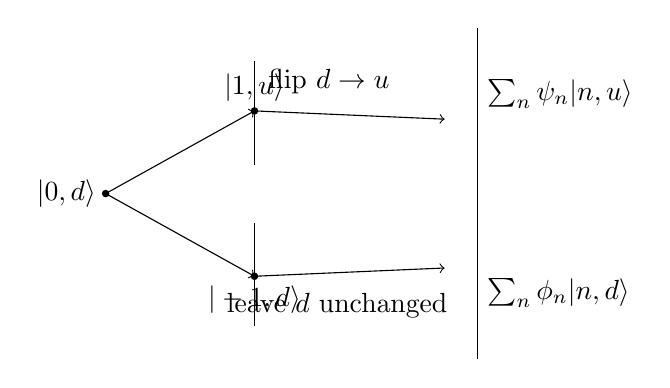
\begin{tikzpicture}[scale=1.05]
\fill (0,0) circle (1.3pt);
\node[left] at (0,0) {$|0,d\rangle$};

\draw (1.8,1.6) -- (1.8,0.35);
\draw (1.8,-0.35) -- (1.8,-1.6);
\fill (1.8,1) circle (1.3pt);
\fill (1.8,-1) circle (1.3pt);
\node[above] at (1.8,1) {$|1,u\rangle$};
\node[below] at (1.8,-1) {$|-1,d\rangle$};

\draw (4.5,2.0) -- (4.5,-2.0);
\node[right] at (4.5,1.2) {$\sum_n \psi_n |n,u\rangle$};
\node[right] at (4.5,-1.2) {$\sum_n \phi_n |n,d\rangle$};

\draw[->] (0,0) -- (1.8,1);
\draw[->] (0,0) -- (1.8,-1);
\draw[->] (1.8,1) -- (4.1,0.9);
\draw[->] (1.8,-1) -- (4.1,-0.9);

\node at (2.7,1.35) {flip \(d\to u\)};
\node at (2.8,-1.35) {leave \(d\) unchanged};
\end{tikzpicture}
\caption{القياس بوصفه تشابكًا مع اللف المغزلي لكاشف. يقلب المسار العلوي اللف المغزلي للجهاز؛ ويتركه المسار السفلي دون تغيير.}
\end{figure}

افترض، كما تفعل المحاضرة، ألا يحدث للّف المغزلي شيء آخر أثناء الرحلة إلى الشاشة. عندئذٍ
\begin{align}
|1,u\rangle &\longrightarrow \sum_n \psi_n |n,u\rangle, \\
|-1,d\rangle &\longrightarrow \sum_n \phi_n |n,d\rangle.
\end{align}
ولذلك تكون الحالة النهائية مع فتح الشقين معًا هي
\begin{equation}
|\Psi_{\mathrm{final}}\rangle
  = \sum_n \psi_n |n,u\rangle + \sum_n \phi_n |n,d\rangle.
\end{equation}
وهذا ليس تراكبًا لحالات إلكترون واحد وحده. بل هو حالة متشابكة للإلكترون والجهاز.

\begin{figure}[htbp]
\centering
\includegraphics[width=0.68\textwidth]{lecture_06_figure_13.png}
\caption{تصل سعتا المسارين إلى الشاشة وهما تحملان سجلين متعامدين للجهاز.}
\lectureframe{01:47:35}
\end{figure}

أنسب طريقة لحساب احتمال الوصول إلى الموضع \(m\) هي استخدام المسقِط على ذلك الموضع في المنظومة الفرعية للإلكترون:
\begin{equation}
\Pi_m = |m\rangle\langle m|\otimes I_{\mathrm{spin}}.
\end{equation}
ويعطي تطبيق \(\Pi_m\) على الحالة النهائية
\begin{equation}
\Pi_m |\Psi_{\mathrm{final}}\rangle
= |m\rangle\bigl(\psi_m|u\rangle+\phi_m|d\rangle\bigr).
\end{equation}
إذن فإن احتمال الوصول إلى \(m\) هو
\begin{align}
P_m
  &= \langle \Psi_{\mathrm{final}}|\Pi_m|\Psi_{\mathrm{final}}\rangle \\
  &= \bigl(\psi_m^*\langle u|+\phi_m^*\langle d|\bigr)
     \bigl(\psi_m|u\rangle+\phi_m|d\rangle\bigr) \\
  &= |\psi_m|^2 + |\phi_m|^2
     + \psi_m^*\phi_m\langle u|d\rangle
     + \phi_m^*\psi_m\langle d|u\rangle.
\end{align}
لكن حالتي السجل متعامدتان:
\begin{equation}
\langle u|d\rangle=0.
\end{equation}
ومن ثم تتلاشى الحدود المتقاطعة:
\begin{equation}
P_m = |\psi_m|^2 + |\phi_m|^2.
\end{equation}
وهذه هي الخلاصة الرياضية الحاسمة في المحاضرة. فبمجرد أن تُسجَّل معلومات أيِّ المسارين، يختفي التداخل وتُجمَع الاحتمالات على الطريقة الكلاسيكية.

\begin{classroomqa}
\lecturetimestamp{01:49:09}
\audiencequestion{ما الفرق بين التراكب \(|1\rangle+|-1\rangle\) والحالة \(|1,u\rangle+|-1,d\rangle\)؟}
\lecturerresponse{الأول يتعلق بمنظومة واحدة في تركيب خطي لموضعين؛ ولا يوجد شيء آخر يمكن أن تكون متشابكة معه. والثاني يتعلق بمنظومتين ويربط المسار بلف الكاشف المغزلي. وعندئذٍ تكشف قراءة اللف المغزلي معلومات عن المسار.}
\end{classroomqa}

\section{السجلات البيئية والقياس الجزئي}

الكاشف المصنوع عمدًا ليس المسجِّل الوحيد. يمكن لذرة قرب شق، أو لغاز متبقٍّ، أو لسطح حراري، أو لأي درجة حرية أخرى أن ترتبط بالمسار. فإذا كانت حالتاها النهائيتان هما \(|E_1\rangle\) و\(|E_2\rangle\)، فإن حالة المسار تأخذ الصورة
\begin{equation}
|\Psi\rangle
=\sum_n\left(\psi_n|n\rangle|E_1\rangle
+\phi_n|n\rangle|E_2\rangle\right).
\end{equation}
وتُضرب حدود التداخل الآن في مقدار التراكب \(\langle E_1|E_2\rangle\). وتجعل السجلات المتعامدة المسارين قابلين للتمييز تمييزًا تامًا وتمحو التداخل بالكامل. أما السجلات المتطابقة فتُبقي \(\langle E_1|E_2\rangle=1\) وتحافظ على التداخل. ويعطي التراكب المتوسط وضوحًا جزئيًا.

\begin{figure}[htbp]
\centering
\includegraphics[width=0.68\textwidth]{lecture_06_figure_14.png}
\caption{توضح الحزم الموجية البيئية المتداخلة والمنفصلة سجلاتٍ جزئية وكاملة للمسار.}
\lectureframe{01:53:40}
\end{figure}

\begin{classroomqa}
\lecturetimestamp{01:50:48}
\audiencequestion{هل يمكن لذرة عادية قرب الشق أن تصبح متشابكة مع الإلكترون المار حتى لو لم يراقبها أحد عن قصد؟}
\lecturerresponse{نعم. ليست المعرفة هي الفعل الحاسم؛ بل الارتباط الفيزيائي. فإذا اضطُربت الذرة أو الغاز المحيط بما يكفي بحيث تميز حالتها اللاحقة المسار، فإنها تسجل معلومات أيِّ المسارين وتثبط التداخل. ولهذا تتطلب مثل هذه التجارب عزلاً ودرجات حرارة منخفضة، وكثيرًا ما تتطلب جسيمات ضعيفة التفاعل مثل الفوتونات.}
\end{classroomqa}

يضع التبريد درجات الحرية البيئية قريبًا من حالاتها القاعية ويقلل السجلات العرضية. كما تساعد فجوة طاقية أيضًا: فإذا لم يستطع الجسيم الساقط أن يزوّد الحد الأدنى من طاقة الإثارة، فقد تعجز البيئة عن الاحتفاظ بمعلومات المسار. وعلى العكس، تستطيع الجسيمات المشحونة أن تزعج المادة القريبة عبر حقولها الكهربائية، مما يجعل تحقيق تداخل الإلكترونات متطلبًا على نحو خاص.

\begin{classroomqa}
\lecturetimestamp{01:54:49}
\audiencequestion{هل يمكن حقًّا الحصول على نمط تداخل بإلكترونات مفردة؟}
\lecturerresponse{يُحدث كل إلكترون ضربة موضعية واحدة فقط. أرسل الجسيمات واحدًا بعد واحد، مع فصل كافٍ بحيث لا تستطيع أن تتفاعل، واجمع عددًا كبيرًا من التكرارات. ويُظهر توزع التواتر المتراكم نمط التداخل؛ أما الحدث الواحد وحده فليس إلا بقعة.}
\end{classroomqa}

\begin{classroomqa}
\lecturetimestamp{01:55:59}
\audiencequestion{هل يدمر القياس التشابك أم ينشئه؟}
\lecturerresponse{إن تفاعل تحديد أيِّ المسارين ينشئ تشابكًا بين المنظومة والجهاز، وهذا التشابك يدمر التداخل بين البديلين. وقد يربط قياس لاحق الجهاز بمنظومة أخرى أيضًا، وقد يجعل الحالة المتبقية مشروطة، لذا يجب دائمًا أن يُذكر أيُّ منظومتين فرعيتين وأيُّ تداخل يجري الحديث عنه.}
\end{classroomqa}

\begin{classroomqa}
\lecturetimestamp{01:57:44}
\audiencequestion{هل يمكن إضعاف التفاعل بحيث لا يحصل الجهاز إلا على معلومات جزئية عن المسار؟}
\lecturerresponse{نعم. فقد يقلب تفاعل ضعيف لفَّ الكاشف المغزلي بسعةٍ ما فقط، تاركًا حالات سجل غير متعامدة. وعندئذٍ لا يكون المساران قابلين للتمييز إلا جزئيًا، ولا يُخفَّض التداخل إلا جزئيًا. والقياس الأقوى يعني قابلية تمييز أكبر، وتشابكًا أقوى مع السجل، ووضوحًا أقل للأهداب.}
\end{classroomqa}

وعليه فالانهيار المعني هنا أمر ملموس: إنه فقدان الحدود المتقاطعة عندما تكون معلومات المسار قد أودعت في منظومة أخرى. ومن دون سجل، تتجمع السعات. ومع سجلات قابلة للتمييز تمييزًا تامًا، ينعدم حاصل ضربها الداخلي وتُجمع الاحتمالات. وبين هذين الحدين، تتغير شدة القياس ووضوح التداخل تغيرًا مستمرًا.
